
\documentclass[aspectratio=169]{beamer}

\usepackage{amsmath,amssymb}
\usepackage{bm}
\usepackage{physics}
\usepackage{tikz}
\usepackage{pgfplots}
\pgfplotsset{compat=1.18}

\title{Von Neumann Stability for FTCS (1D Heat Equation)}
\subtitle{Why Fourier modes, amplification factors, and the $\lambda \le \tfrac12$ restriction}
%\author{Mike Gosz}
\date{}

\begin{document}

% ------------------------------------------------------------
\begin{frame}
  \titlepage
\end{frame}

% ------------------------------------------------------------
\begin{frame}{What ``stability'' means for time stepping}
A time-stepping method is \emph{stable} if small perturbations (round-off, truncation, imperfect data)
remain bounded as the computation advances.

\vspace{0.5em}
For diffusion problems, stable schemes typically \emph{damp} perturbations; unstable schemes may amplify them
until they dominate the solution (nonphysical oscillations / blow-up).
\end{frame}

% ------------------------------------------------------------
\begin{frame}{Model problem and FTCS update}
1D heat equation (no source):
\begin{equation}
\frac{\partial T}{\partial t} = \alpha \frac{\partial^2 T}{\partial x^2}.
\end{equation}

Uniform grid with spacing $\Delta x$ and time step $\Delta t$.
Define
\[
\lambda = \frac{\alpha \Delta t}{(\Delta x)^2}.
\]

FTCS update (interior points):
\begin{equation}
T_j^{n+1} = (1-2\lambda)\,T_j^n + \lambda\left(T_{j+1}^n + T_{j-1}^n\right).
\end{equation}
\end{frame}

% ------------------------------------------------------------
\begin{frame}{Big picture: why Fourier modes}
Key idea (from the notebook):
\begin{itemize}
  \item Any (reasonable) grid temperature profile can be written as a \textbf{sum of Fourier modes}.
  \item FTCS is \textbf{linear} with \textbf{constant coefficients} $\Rightarrow$ it advances \textbf{each mode independently}.
  \item For a single mode, one step multiplies its amplitude by an \textbf{amplification factor}
  \begin{equation}
    G(\theta)=\frac{A^{n+1}}{A^n}.
  \end{equation}
  \item Stability requires \textbf{no mode grows}: $|G(\theta)|\le 1$ for all $\theta \in [0,\pi]$.
\end{itemize}
\end{frame}

% ------------------------------------------------------------
\begin{frame}{A single Fourier mode on a grid}
Assume a Fourier mode on the grid:
\begin{equation}
T_j^n = A^n\, e^{i\theta j},
\end{equation}
where $\theta$ is the nondimensional wavenumber (phase advance per grid point).

\vspace{0.5em}
\textbf{Interpretation:}
\begin{itemize}
  \item $j$ labels grid points.
  \item The mode oscillates in space; $A^n$ carries the time dependence.
\end{itemize}
\end{frame}

% ------------------------------------------------------------
\begin{frame}{Real temperature fields and conjugate pairs}
A real-valued temperature field is built from conjugate pairs:
\[
A_m e^{ik_m x} + A_m^{*} e^{-ik_m x} \;\;\in \mathbb{R}.
\]

Equivalently on a grid:
\[
A\,e^{i\theta j} + A^{*}e^{-i\theta j} = 2\Re(A)\cos(\theta j) - 2\Im(A)\sin(\theta j).
\]

\vspace{0.5em}
\textbf{Takeaway:} complex exponentials are a convenient algebra tool; real solutions come from taking the real part
(or using cosine/sine series).
\end{frame}

% ------------------------------------------------------------
\begin{frame}{Superposition: building an arbitrary profile}
A general profile on $N$ grid points can be written as a sum of modes:
\[
T_j = \sum_{m=0}^{N-1} A_m e^{i\theta_m j}, \qquad \theta_m = \frac{2\pi m}{N}.
\]

In practice, a truncated sum often captures the main shape:
\[
T_j \approx A_0 + \sum_{m=1}^{M} \left(\tilde a_m\cos(\theta_m j) + \tilde b_m\sin(\theta_m j)\right).
\]

\vspace{0.5em}
\textbf{Notebook demo:} a smooth ``bump'' can be reconstructed by adding a handful of low-frequency modes.
\end{frame}

% ------------------------------------------------------------
\begin{frame}{Plug the mode into FTCS}
Insert $T_j^n = A^n e^{i\theta j}$ into
\[
T_j^{n+1} = (1-2\lambda)T_j^n + \lambda(T_{j+1}^n + T_{j-1}^n).
\]

You get:
\[
A^{n+1}e^{i\theta j} =
(1-2\lambda)A^n e^{i\theta j}
+ \lambda A^n\left(e^{i\theta(j+1)} + e^{i\theta(j-1)}\right).
\]

Divide by $A^n e^{i\theta j}$:
\begin{equation}
\frac{A^{n+1}}{A^n} = 1 + \lambda\left(e^{i\theta} - 2 + e^{-i\theta}\right).
\end{equation}
\end{frame}

% ------------------------------------------------------------
\begin{frame}{Simplify the exponentials}
Use Euler's identity:
\[
e^{i\theta} + e^{-i\theta} = 2\cos\theta.
\]

So
\[
e^{i\theta} - 2 + e^{-i\theta} = 2\cos\theta - 2 = 2(\cos\theta - 1).
\]

Therefore,
\begin{equation}
\boxed{
G(\theta)=\frac{A^{n+1}}{A^n} = 1 + 2\lambda(\cos\theta - 1)
= 1 - 4\lambda \sin^2\!\left(\frac{\theta}{2}\right).
}
\end{equation}
\end{frame}

% ------------------------------------------------------------
\begin{frame}{Stability condition and worst-case mode}
Stability requires:
\[
|G(\theta)| \le 1 \quad \text{for all } \theta\in[0,\pi].
\]

Since $\sin^2(\theta/2)\in[0,1]$, the most restrictive case is the highest-frequency grid mode:
\[
\theta=\pi \quad \Rightarrow\quad \sin^2\!\left(\frac{\theta}{2}\right)=1.
\]

Then
\[
G(\pi)=1-4\lambda.
\]

Require $-1\le G(\pi)\le 1$:
\[
-1 \le 1 - 4\lambda \;\Rightarrow\; \lambda \le \frac{1}{2}.
\]

\[
\boxed{\Delta t \le \frac{(\Delta x)^2}{2\alpha}}
\]
\end{frame}

% ------------------------------------------------------------
\begin{frame}{Visual: $G(\theta)$ vs.\ $\theta$}
\centering
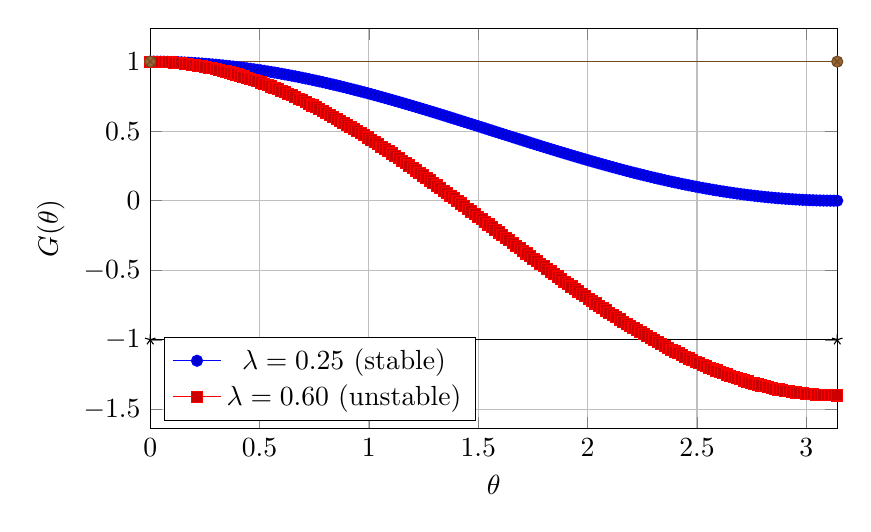
\begin{tikzpicture}
\begin{axis}[
  width=0.85\textwidth,
  height=0.55\textwidth,
  xlabel={$\theta$},
  ylabel={$G(\theta)$},
  xmin=0, xmax=3.14159,
  ymajorgrids=true,
  xmajorgrids=true,
  legend style={at={(0.02,0.02)},anchor=south west},
]
\addplot+[domain=0:3.14159, samples=200] {1 + 2*0.25*(cos(deg(x)) - 1)};
\addlegendentry{$\lambda=0.25$ (stable)}
\addplot+[domain=0:3.14159, samples=200] {1 + 2*0.60*(cos(deg(x)) - 1)};
\addlegendentry{$\lambda=0.60$ (unstable)}
\addplot+[domain=0:3.14159, samples=2] {1};
\addplot+[domain=0:3.14159, samples=2] {-1};
\end{axis}
\end{tikzpicture}

\vspace{-0.25em}
Stable requires the entire curve to stay between $-1$ and $+1$.
\end{frame}

% ------------------------------------------------------------
\begin{frame}{Notebook figure: single mode stays a single mode}
\textbf{What the notebook shows:}
\begin{itemize}
  \item Start with a single Fourier mode $T_j^0$ (blue).
  \item After $n$ steps, FTCS gives
  \[
  T_j^n = G(\theta)^n T_j^0,
  \]
  so the \textbf{shape is unchanged} and the \textbf{amplitude scales} by $G(\theta)^n$.
  \item If $|G(\theta)|<1$ the mode decays; if $|G(\theta)|>1$ it grows.
\end{itemize}

\vspace{0.5em}
\textbf{Takeaway:} von Neumann stability is about ensuring \emph{every} Fourier mode decays (or at least does not grow).
\end{frame}

% ------------------------------------------------------------
\begin{frame}{Connecting back to engineering intuition}
\begin{itemize}
  \item Diffusion should smooth the solution $\Rightarrow$ high-frequency content should decay fastest.
  \item FTCS is explicit: too large $\Delta t$ causes the discrete update to overreact.
  \item The most dangerous mode is the grid-scale oscillation ($\theta=\pi$): alternating $+/-$ from node to node.
\end{itemize}

\vspace{0.5em}
\textbf{Design rule:}
\[
\Delta t \le \frac{(\Delta x)^2}{2\alpha}
\quad\Rightarrow\quad
\text{refine grid} \;(\Delta x \downarrow)\; \Rightarrow\; \Delta t \downarrow \text{ quadratically.}
\]
\end{frame}

% ------------------------------------------------------------
\begin{frame}{Summary}
\begin{itemize}
  \item Assume a Fourier mode $T_j^n = A^n e^{i\theta j}$.
  \item FTCS advances each mode independently:
  \[
  \frac{A^{n+1}}{A^n}=G(\theta)=1+2\lambda(\cos\theta-1).
  \]
  \item Stability requires $|G(\theta)|\le 1$ for all $\theta$.
  \item Worst case $\theta=\pi$ gives:
  \[
  0\le \lambda \le \frac12 \quad\Longleftrightarrow\quad \Delta t \le \frac{(\Delta x)^2}{2\alpha}.
  \]
\end{itemize}
\end{frame}

\end{document}
